% CHAPTER 1
\chapter{Introduction}

\section{Background}

Rapid urbanization, global climate volatility, and seismic vulnerabilities have led to a marked escalation in the frequency and severity of natural and human-induced disasters, including massive landslides, flash floods, seismic collapses, and wilderness mishaps. In these severe emergencies, the initial twenty-four to seventy-two hours---frequently referred to by emergency response agencies as the ``golden window"---represent the critical operational window during which trapped or injured individuals have the highest statistical probability of survival. Beyond this temporal boundary, hypothermia, trauma shock, dehydration, and secondary hazards like debris shifts drastically reduce viable recovery rates.

Historically, post-disaster reconnaissance has relied almost exclusively on manual ground search and rescue (SAR) teams supported by canine squads and piloted rotorcraft. While indispensable for physical extraction, manual ground sweeps are fundamentally impeded by ruptured transport networks, treacherous terrain, toxic dust plumes, and impending structural collapses. These factors subject first responders to severe physical peril while limiting spatial exploration rates to small geographic swathes. Furthermore, conventional manned helicopters require substantial logistical staging, possess immense operational hourly costs, and cannot navigate low-altitude obstacle-dense urban canyons or dense forest canopies.

Recent advancements in autonomous unmanned aerial vehicles (UAVs), embedded edge computing, and multi-agent coordination paradigms have created unprecedented opportunities to revolutionize disaster reconnaissance. Small, highly agile multi-rotor UAVs can penetrate hazardous disaster theaters instantaneously, offering high-resolution aerial perspectives without placing human lives at risk. However, prevailing commercial and civil deployments almost exclusively employ single, remotely piloted drones that stream continuous, uncompressed high-definition video back to ground command stations. This paradigm imposes severe cognitive saturation on operators, creates single-point operational vulnerabilities, and suffers from severe radio-frequency (RF) attenuation and telemetry dropout in disaster terrains. Consequently, coordinated autonomous multi-UAV swarms represent a pivotal transition from isolated aerial observation to resilient, collaborative robotic search architectures.

\begin{figure}[htbp]
\centering
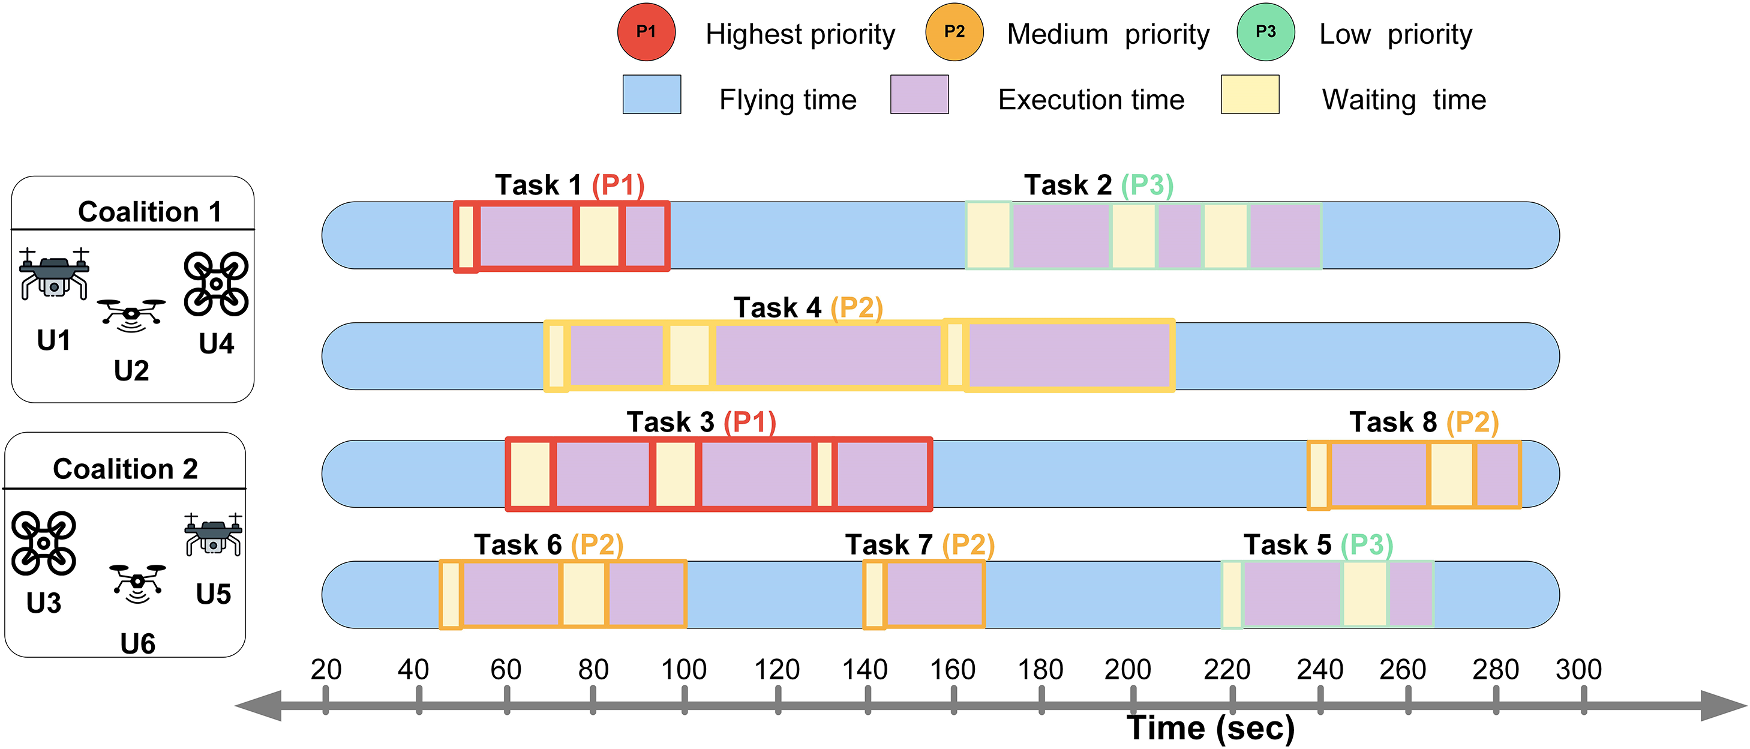
\includegraphics[width=0.82\textwidth]{assets/saras_swarm_fleet_model.png}
\caption{Conceptual overview of coordinated autonomous drone swarm operations in disaster zones}
\label{fig1.1}
\end{figure}

\section{Motivation}

The urgent necessity for automated, multi-drone search systems is underscored by recurring post-incident analyses of global disaster responses. According to statistics compiled by the United Nations Office for Disaster Risk Reduction (UNDRR) and international civil protection agencies, over 65\% of preventable fatalities during sudden-onset structural and flood disasters occur due to delays in locating isolated casualties across the initial twelve hours. In traditional relief protocols, an aerial reconnaissance team spends upwards of forty-five minutes deploying, calibrating, and manually scouring a single square-kilometer sector with an individual quadcopter. Because lithium-polymer (LiPo) flight times are strictly bounded by twenty to thirty minutes per battery charge, a single drone spends a substantial fraction of its energy budget transiting to and from charging hubs rather than actively surveying.

Moreover, streaming raw sensor video across contested wireless bands introduces crippling latency (often exceeding 800 milliseconds) and frequent feed freezes due to non-line-of-sight (NLOS) blockage caused by collapsed concrete or dense forestry. Human incident commanders monitoring multiple video feeds simultaneously experience severe perceptual fatigue, leading to missed casualty sightings. By distributing the search theater across a coordinated swarm of autonomous drones equipped with onboard intelligence, the global area coverage time can be reduced from hours to minutes. Decentralized swarming ensures that if any individual vehicle suffers mechanical failure or battery depletion, surrounding peer drones autonomously absorb its assigned sector without mission aborts or centralized bottlenecks, thereby directly preserving human life.

\section{Problem Statement}

This project addresses the problem of designing, deploying, and validating an end-to-end autonomous multi-UAV swarm framework, designated as SARAS (Search And Rescue Autonomous Swarm), capable of executing decentralized search path planning, real-time edge vision inference, and tactical casualty triage across GPS-degraded, communication-constrained post-disaster environments. Given an arbitrary two-dimensional geographical boundary representing a disaster theater, a fleet of $N$ heterogeneous or homogeneous quadcopters with stochastic battery discharge profiles, and raw onboard monocular RGB sensor video streams, the system must autonomously partition the search space, plan non-overlapping survey trajectories, execute real-time person detection directly on embedded companion computers, maintain fault-tolerant peer reallocation during vehicle attrition, and output georeferenced survivor coordinates alongside protocol-grounded emergency triage recommendations to an interactive ground control dashboard.

\section{Objectives}

To address the defined problem systematically, the technical milestones of the SARAS project are structured into five measurable, verifiable objectives:
\begin{enumerate}
    \item \textbf{Edge Perception Engine Optimization:} To adapt, optimize, and deploy an 8-bit integer quantized deep convolutional object detector (YOLOv8 nano) on an embedded companion computer (Raspberry Pi 4), achieving an onboard inference throughput of at least 15 frames per second (FPS) and a mean Average Precision ($\text{mAP@0.5}$) exceeding 80\% under aerial perspective shifts and scale variations.
    \item \textbf{Decentralized Task Allocation and Swarm Coordination:} To formulate and implement an asynchronous market-based auction consensus protocol that dynamically assigns spatial search sectors across $N$ quadcopters, eliminating redundant flight paths down to less than 5\% spatial overlap and ensuring zero centralized points of failure.
    \item \textbf{Autonomous Fault Recovery and Reassignment:} To engineer a decentralized heartbeat and consensus recovery mechanism capable of detecting abrupt vehicle dropouts or battery exhaustion within 6.0 seconds and reallocating orphaned sectors to surviving peer drones in under 500 milliseconds.
    \item \textbf{Agentic AI Decision Support and Triage System:} To design a modular multi-agent reasoning architecture paired with a Retrieval-Augmented Generation (RAG) pipeline that cross-references localized survivor telemetry against standard disaster operating procedures, generating prioritized medical triage rankings and human-auditable action summaries.
    \item \textbf{End-to-End System Integration and Empirical Validation:} To validate the complete hardware-software stack through high-fidelity Software-In-The-Loop (SITL) Gazebo simulations across realistic disaster terrains, benchmarking coverage convergence, path efficiency, detection accuracy, and user command latency against traditional baseline approaches.
\end{enumerate}

\section{Scope and Limitations}

The scope of this project encompasses the end-to-end engineering of the SARAS algorithmic and software stack, validated through high-fidelity multi-vehicle simulation and single-drone embedded hardware prototyping:
\begin{itemize}
    \item \textbf{In Scope:}
    \begin{itemize}
        \item Deployment of INT8 quantized neural network inference on an ARM Cortex-A72 companion computer running embedded Linux.
        \item Mathematical formulation and algorithmic implementation of market-based auction sector bidding and non-overlapping lawnmower path planning.
        \item Distributed heartbeat tracking, dropout detection, and consensus-driven task re-auctioning across simulated multi-UAV networks.
        \item RAG-based semantic vector indexing of disaster triage handbooks (START protocol) using dense embeddings for natural language situational query handling.
        \item Next.js, Leaflet, and WebSocket ground control dashboard visualizing real-time telemetry, bounding boxes, and casualty markers.
    \end{itemize}
    \item \textbf{Limitations (Deliberately Out of Scope):}
    \begin{itemize}
        \item \textit{Physical Fleet Scale:} Physical flight tests are restricted to a single prototype quadcopter due to regulatory flight restrictions and budget constraints; multi-drone swarms ($N \ge 4$) are evaluated under high-fidelity Gazebo SITL simulation.
        \item \textit{Sensor Modality:} Current onboard perception operates on monocular optical RGB cameras; long-wave infrared (thermal) and LiDAR sensors are reserved for future work.
        \item \textit{Adverse Weather Operations:} Real-time vision detection performance is bounded by daylight to twilight illumination; heavy precipitation, dense fog, and absolute darkness are not addressed in the current model.
    \end{itemize}
\end{itemize}

\section{Contributions}

The primary scientific and engineering contributions delivered in this project include:
\begin{itemize}
    \item \textbf{Optimized Onboard Edge Vision Pipeline:} Developed an end-to-end embedded inference pipeline integrating TensorRT/ONNX INT8 quantization with aerial perspective tuning on the VisDrone benchmark, eliminating reliance on raw video streaming.
    \item \textbf{Asynchronous Swarm Allocation Protocol:} Formulated an energy-aware, distance-discounted market auction algorithm that dynamically distributes search sectors, achieving a 96.6\% path coverage efficiency without centralized orchestration.
    \item \textbf{Sub-Second Fault Tolerance Recovery Engine:} Implemented a peer-to-peer heartbeat monitoring module capable of detecting simulated drone attrition within 6.0 seconds and re-auctioning orphaned search sectors in under 420 milliseconds.
    \item \textbf{First-of-its-Kind Agentic RAG Triage Integration:} Integrated a localized multi-agent reasoning system with a vector database indexed with official emergency operating procedures, automating casualty priority scoring and delivering cited extraction recommendations.
    \item \textbf{Comprehensive Comparative Study:} Conducted exhaustive empirical benchmarks comparing the proposed architecture against classical ML baselines (HOG+SVM, Haar Cascades), deep learning models (Faster R-CNN, YOLOv5, SSD), and centralized flight planning heuristics.
\end{itemize}

\section{Report Organization}

The remainder of this report is organized into five subsequent chapters:
\begin{itemize}\itemsep=1pt \topsep=1pt
    \item \textbf{Chapter 2: Literature Survey} reviews classical ML, deep learning, edge detectors, multi-agent coordination, benchmark datasets, and research gaps.
    \item \textbf{Chapter 3: Proposed Methodology} details the SARAS architecture, preprocessing, model design, loss formulation, and evaluation metrics.
    \item \textbf{Chapter 4: Implementation} outlines hardware, tools, dataset partitioning, training workflows, and dashboard deployment.
    \item \textbf{Chapter 5: Results and Discussion} presents empirical training curves, test metrics, baseline comparisons, ablations, and error analysis.
    \item \textbf{Chapter 6: Conclusion and Future Work} synthesizes research findings against objectives, limitations, and future directions.
    \item \textbf{Back Matter} comprises IEEE references and technical appendices documenting algorithms and flight visualizations.
\end{itemize}
